\documentclass[11pt]{article}

%% \usepackage{deauthor,times,graphicx}
%% \usepackage{hyperref}
%% \usepackage{xcolor}
%% \usepackage{comment}

%% \graphicspath{{figs/}}
%% \begin{document}

%% \title{A Bird’s Eye View of the 4th Industrial Revolution Technologies}
%% \author{Kyu-Young Whang$^{1,2}$, Jae-Gil Lee$^2$, Hyo-Sang Lim$^3$, Inju Na$^2$ \\
%% $^1$National Academy of Sciences Republic of Korea \\
%% $^2$KAIST \\
%% $^3$Yonsei University, Wonju \\
%% {\small \{kywhang, jaegil, ijna\}@kaist.ac.kr, hyosang@yonsei.ac.kr}}
\begin{document}
%% \maketitle

\section{Introduction}

Big data and artificial intelligence\,(AI) are at the core of the rapid digitalization of all aspects in our lives, which is referred to as the Digital Transformation, 4th Industrial Revolution, or Industry 4.0. In particular, the term ``4th Industrial Revolution (4IR)'' proposed by Klaus Schwab, the founder of the World Economic Forum, is widely used in the scientific literature. As significant parts of our work and personal life are now performed non-face-to-face due to the COVID-19 crisis, the development of 4IR technologies has been accelerating. At the same time, it is difficult to understand and digest all the new 4IR technologies that are pouring out every day. 
With this motivation, we take a bird's eye view of exploring these technologies and their relationships (Section 2). We then elaborate on the base and core technologies (Sections 3 and 4) and a key application (Section 5). 
%With this motivation, we examine the structure of these technologies from a bird’s eye view to see what they look like in a large framework and identify their relationships in Section 2. Then, we briefly discuss on base and core technologies in Sections 3 and 4.  Finally, we introduce an example application technology in Section 5.
 
\subsection{Definition of Industrial Revolution}
An industrial revolution occurs when impactful new technologies cause rapid changes in industrial and manpower structures, which in turn cause large economic and social changes. The 1st Industrial Revolution refers to the drastic economical and societal changes caused by technological innovations and transitions to new manufacturing processes triggered by James Watt’s steam engine, which was invented in the mid-18th and early 19th centuries. The 2nd Industrial Revolution generally refers to innovative changes triggered by the use of electricity and oil, which was made possible by Thomas Edison, Nicola Tesla, and George Westinghouse at the end of the 19th century. The 3rd Industrial Revolution, which is also called the Digital Revolution or Information Revolution, mainly refers to the large economic and social changes triggered by the advent of computers and the Internet at the end of the 20th century. The term ``3rd Industrial Revolution’’ was first used by Jeremy Rifkin in his 2011 book with the same title\,\cite{Rifkin2011}. The 4th Industrial Revolution was first mentioned in 2016 at the World Economic Forum (WEF, aka Davos Forum) chaired by Klaus Schwab\,\cite{Schwab2016}. There are various definitions for 4IR. 
% In essence, we are witnessing economic and social (even political) changes that are caused by intelligent processes using Big data and AI in a world where all people and things are increasingly connected globally in real time starting from the 21st century. 
The fusion of the physical, digital, and biological worlds claimed in 4IR is expected to be realized through metaverse technology.
% , and its development is accelerating due to widespread lifestyle changes caused by the COVID-19 pandemic. 
Notably, Facebook has changed its company name to Meta and is working to dominate the technology market. Being confined to the manufacturing sector, digital transformation characterized by AI, big data, and the Internet of Things\,(IoT) is combined with robot technology to lead to automation of existing production processes. In the EU, centering on Germany, technology development for a smart factory is collectively referred to as ``Industry 4.0''\,\cite{lasi2014industry}.
Some including Jeremy Rifkin view this process as a continuation of the 3rd Industrial Revolution. However, it appears that, while the 3rd Industrial Revolution has an emphasis on improved productivity through fast computation and improved communication through the Internet, 4IR focuses on intelligence including AI (especially, deep learning) that may replace humans and on the integration of %The Fourth Industrial Revolution refers the fusion of technologies across the physical, digital and biological worlds 
real and virtual worlds in a hyper-connected society\,\cite{Schwab2016b}. In particular, the metaverse is increasingly becoming a reality especially due to COVID-19 where many conferences are held virtually and people are interacting through avatars. In addition, more and more virtual and augmented reality\,(VR/AR) products are becoming available.

\subsection{Impact of Industrial Revolution}
As mentioned above, an industrial revolution introduces innovative new technologies, which cause sudden industrial structure changes and impact the job market. The major issues for such a rapid change are the lack of manpower for the new industry and the long time it takes to train a workforce. At the same time, large-scale unemployment is expected of many workers/experts of the existing industry due to its rapid decline. High-tech industries are no exception. In the automobile industry, for example, a significant portion (30--50\%) of new car sales is expected to be filled with electric vehicles made with simpler processes within the next decade or so\,\cite{Reuters2022,Hyundai2022}, so the demand for workers in automobile factories, high-tech engine and transmission engineers, and various automobile parts may decrease significantly. Instead, battery and self-driving AI software technologies are expected to replace the existing ones.

Therefore, the following preparations for 4IR are necessary:
\begin{enumerate}
\item Job creation by understanding, leading the development of, and industrializing new technologies for 4IR.
\item Resolving the demand for manpower by systematically nurturing manpower necessary for new industry.
\item Relieving unemployment and demand for manpower through re-education of old-industry professionals.
\end{enumerate}

\section{4IR Technologies and Their Relationships}

We categorize and organize the technologies for 4IR as follows.  Figure 1 shows the result and their relationship in a large framework.

\begin{figure}[h]
  \centering
  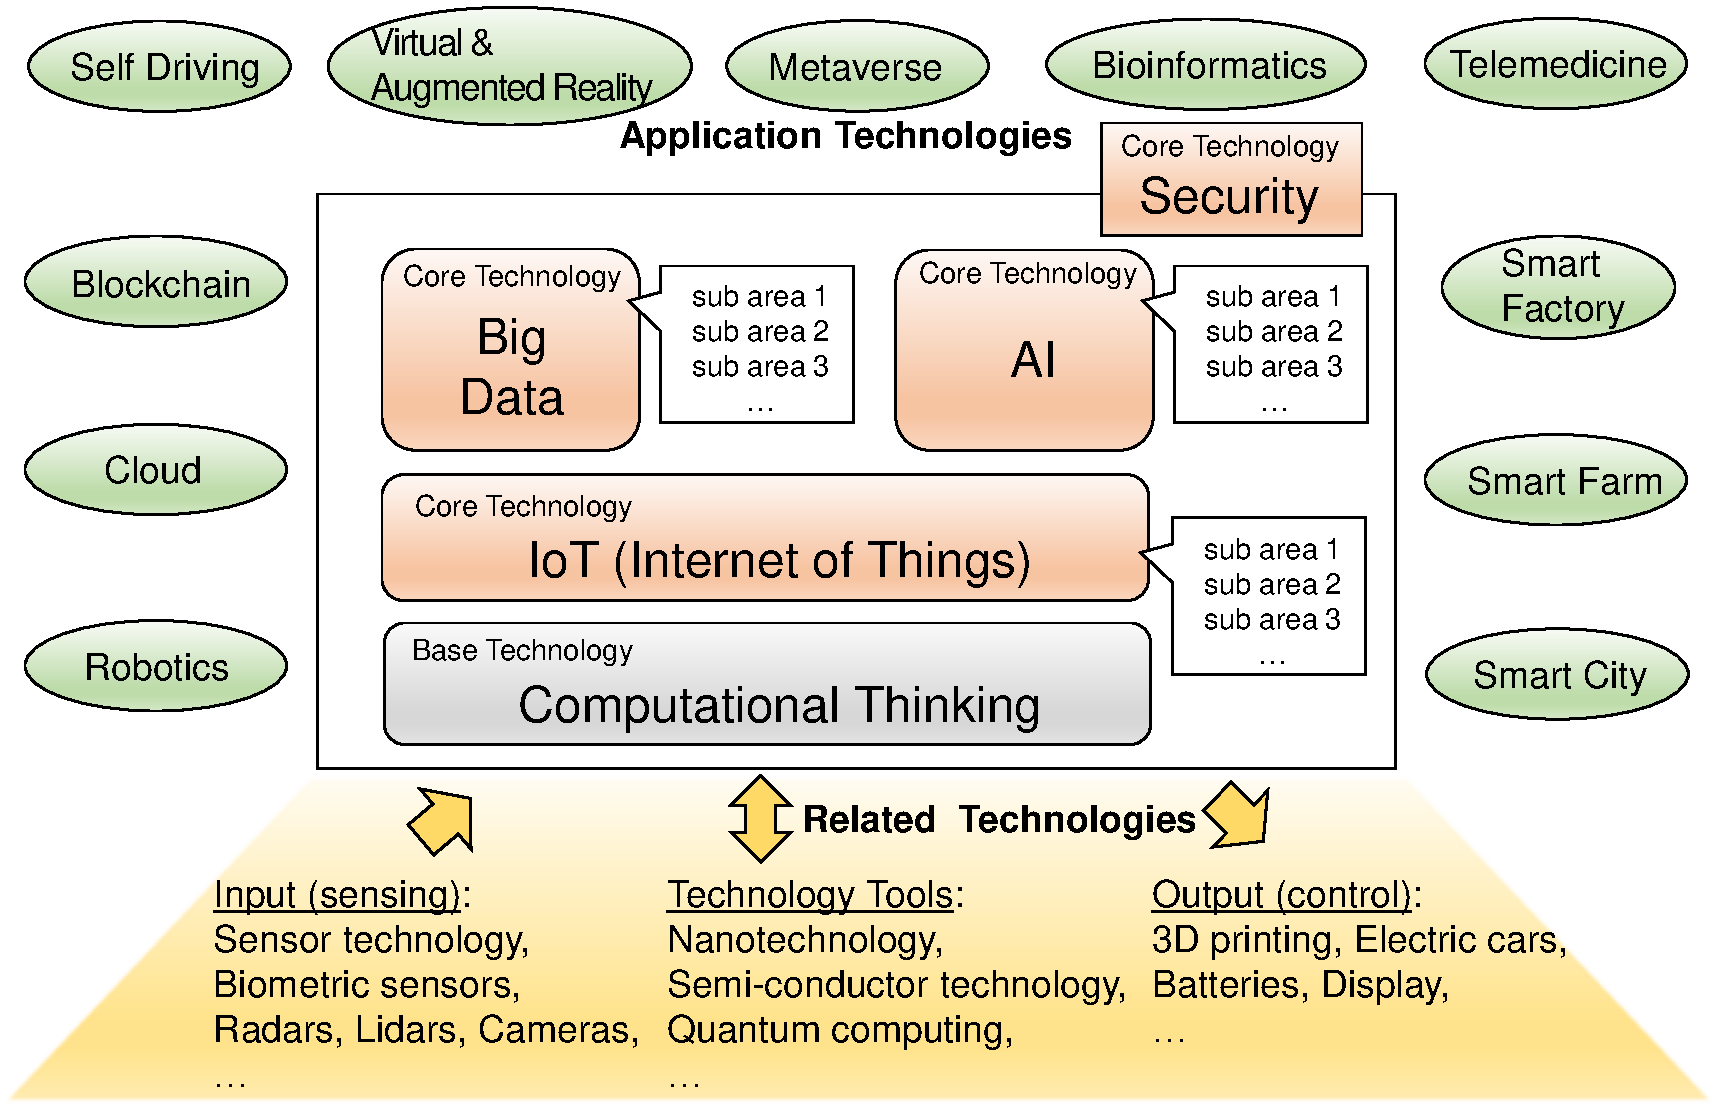
\includegraphics[width=\textwidth]{4IR.pdf}
  \caption{A Bird's eye view of the 4th Industrial Revolution technologies and their relationships.}
  \label{fig:4ir}
\end{figure}

\subsection{Core Technologies}
At the core is a hyper-connected network that can be envisioned as one giant computer. The operations of this computer are sensing, computing, and control/interaction for integrating real and virtual worlds. Big data and AI represent the computing, and the IoT plays the role of the infrastructure. There are also security technologies that protect all these processes. Although not shown here, computer systems form the underlying infrastructure.

\subsection{Base Technologies}
At the base of this paradigm lies computational thinking, which attempts to solve real-life problems computationally. Computational thinking is a fundamental skill required of everyone and not only of computer scientists\,\cite{DBLP:journals/cacm/Wing06}, especially in the 4IR era. Thus, we categorize computational thinking as the base technology, although it may be more appropriate to categorize it as a skill or an approach.

\subsection{Application Technologies}
In Figure 1, example application technologies (by no means exhaustive) based on the core technologies are shown outside the large box and include self driving, VR/AR, metaverse, robotics, smart farms, telemedicine, smart factories, and blockchain. These technologies are already revolutionizing the entire industry. The list is certainly not exhaustive and will keep on growing as AI has become democratized where it is now easy to add intelligence to any existing domain by utilizing open machine learning (ML) platforms such as Google’s TensorFlow and Meta’s PyTorch.

\subsection{Related Technologies}
The related technologies to connect the computer with the real world include various sensor technologies including biometric sensors, radars, lidars, and cameras for the input (sensing part) and 3D printing, electric vehicles, batteries, and display technologies for the output (control/interaction part). Besides, nanotechnology, semi-conductor technology, and quantum computing are widely used for realizing the core technologies as well as the other related technologies. 

In the next sections, we briefly discuss on the core and base technologies and introduce an example application technology on how AI\,(ML) is used in molecular biology, which is a typical approach in bioinformatics. The other application and related technologies are vast, and there are ample opportunities to learn about them through various other media.

% [Add more details on the example application technology in a new section 5]


\section{Base Technology of 4IR}

\subsection{Computational Thinking}
In the 4IR characterized by the metaverse, not only computer scientists, but also general consumers and citizens must be armed with computational thinking. Many countries including the United States, England, and Germany have steadily been revamping their curriculums starting from as early as elementary school (K-12) to strengthen Computer Science education and even require computational thinking\,\cite{10.1145/1929887.1929905,Berry14,DBLP:books/sp/17/DelckerI17,DBLP:books/sp/RH2017}. 
%The International Society for Technology in Education recently defined computational thinking as students “develop[ing] and employ[ing] strategies for understanding and solving problems in ways that lever age the power of technological methods to develop and test solutions” (http://www.iste.org/standards/standards/for-students-2016). 
A pioneering example is the 2014 U.K. educational reform where the subject ``Computing'' was introduced as compulsory in the K-12 curriculum instead of the conventional ICT subject so as to teach students computational thinking, in effect replacing ``how to use'' computers with ``how to be creative'' to understand and change the world\,\cite{Berry14}. 
\emph{Computational thinking} is a methodology ``for understanding and solving problems in ways that leverage the power of technological methods to develop and test solutions''\,\cite{iste2016}.
An alternative description is a set of problem-solving methods that involve formulating problems and solving them in such a way that a computer could also execute\,\cite{wiki-computational-thinking}. 
The four key techniques to computational thinking are decomposition, pattern recognition, abstraction, and algorithms\,\cite{BBC2022}. It involves formulating a problem through summarizing and abstracting a real-world problem and solving it by using an algorithm. During this process, a large problem can be decomposed into smaller problems and solved (divide and conquer). If we borrow the notion ``algorithms + data structures = programs'' by Niklaus Wirth\,\cite{Wirth1976}, computational thinking in short is an approach of solving real life problems by thinking, understanding, analyzing, designing, and executing by computer programs (or computationally).
Since computational thinking constitutes the most basic education to confront 4IR, we categorize it as the base technology.\footnote{Of course some critics worry about ``computational chauvinism''\,\cite{DBLP:journals/cacm/DenningTY17} because computational thinking may not be broad enough to solve all real-life problems.}

\section{Core Technologies of 4IR}

\subsection{AI, Big Data, and Their Integration}

\subsubsection{Integrated Research}
Big data research has been conducted since the 1960’s under the names of file systems, databases, data mining, big data analytics, big data systems, and data science. In the big data era, data has become extremely valuable and is considered to be the oil of the 21st century. Data is also the essential fuel for AI\,(ML). As a result, the collection, storage, processing, and analysis of data has become an indispensable element in any application. AI has been studied since the 1940’s and mimics the human ability to learn, solve problems, and recognize patterns in the form of computer programs. ML is an important branch of AI that uses big data to automatically learn and improve computer algorithms without explicit programming. Platforms such as Google’s TensorFlow have been made public, so the general public can easily use ML in various applications. Applications include self-driving cars, intelligent assistants, AI speakers, AI clerks in marts, automatic defect detection of products in manufacturing, and even professional tasks conducted by doctors and lawyers.
As AI and in particular deep learning heavily rely on large amounts of data, the big data and AI disciplines are becoming increasingly integrated. Within an AI system, ML algorithms account for only a small fraction of all the components in terms of lines of code\,\cite{DBLP:conf/nips/SculleyHGDPECYC15}. In addition to ML code, the significant components include data collection, data verification, feature extraction, and analysis tools. Moreover, according to practitioners of ML, 80--90\% of the efforts in an ML life cycle is spent on data preparation, and many companies have difficulty adopting deep learning due to the need of large amounts of labeled data and the lack of explainability of the trained models\,\cite{DBLP:journals/debu/StonebrakerR19}. In addition, the broad field of data science is not just about ML, but also data mining and database techniques\,\cite{DBLP:journals/debu/Ullman20}. Most recently, even the ML community has started to focus on improving the data for AI performance. Unlike traditional AI where the ML algorithm is of primary interest, the goal is to improve the data while using the same algorithm. This paradigm has been coined as \emph{data-centric AI}\,\cite{data-centric-ai}. In the next sections, we explain two directions of integration: DB to ML and ML to DB.

\subsubsection{DB to ML}
The ML data lifecycle consists of many steps including data understanding, data validation and cleaning, and data preparation\,\cite{DBLP:journals/sigmod/PolyzotisRWZ18}. We summarize how database and data management techniques are being used for these steps.
Better data management can improve ML. For example, data normalization is a common technique to reduce redundancies and anomalies and has been proposed to factorize and improve the speed of ML training as well\,\cite{DBLP:journals/pvldb/ChenKNP17}. Data cleaning has recently been extended and evaluated with the new objective of improving ML accuracy\,\cite{DBLP:conf/icde/LiRBZCZ21}, and data validation techniques are routinely used to check the quality of training data\,\cite{DBLP:conf/kdd/BaylorBCFFHHIJK17}. ML systems are increasingly becoming declarative as well by using schemas and declarative interfaces\,\cite{DBLP:journals/cacm/MolinoR22}. In supervised learning, models are trained using labeled data, and a significant bottleneck is to perform the labeling itself. Data programming\,\cite{DBLP:journals/vldb/RatnerBEFWR20} has been proposed as a way to semi-automatically perform data labeling on unlabeled data where training on large amounts of such data can result in better model accuracy than using smaller amounts of manually-labeled data. 
Another approach is to develop techniques for collecting more datasets that can improve the current training data and lead to better model performance\,\cite{DBLP:journals/tkde/RohHW21}. 
There are new directions in AI that can benefit from data management techniques as well. In particular, \emph{Responsible AI} (also known as \emph{Trustworthy AI}) has become important due to the widespread usage of AI. In addition to simply aim for high accuracy, it is also important to be responsible and guarantee fairness, robustness, privacy, explainability, and transparency among others\,\cite{trustworthy-ai}. \emph{Model fairness} is about removing or coping with bias in the data, which may lead to discriminative predictions\,\cite{compas}. \emph{Robustness} is about ensuring high model accuracy against various noise or poisoning in the data by either removing or fixing them\,\cite{DBLP:conf/icml/SongK019}. \emph{Privacy} is also becoming important as illustrated by a Korean AI chatbot\,\cite{leeluda}, which was famously shut down due to its hate speech and personal information leakage including home addresses. \emph{Explainability} is another important direction where models must be more transparent and understandable when making predictions. Many of these problems can be traced to the training data, so better data management can be a fundamental solution. 

\subsubsection{ML to DB}
The other direction, ML to DB, has been extensively studied recently\,\cite{DBLP:journals/debu/KraskaM0PPRS21}. In this direction, ML techniques are used to improve the performances of various components of a DBMS including indexing, query optimization, and parameter tuning. An index like a B-tree or hash table can be viewed as a function receiving a key attribute value as an input and returning a location of the record with that value. This function can also be learned from data by training a model that is smaller than the index and can be looked up faster\,\cite{DBLP:conf/sigmod/DingMYWDLZCGKLK20}. Query optimization involves searching for the most efficient query plan, and reinforcement learning is a suitable technique as it can help speed up the searching without having to perform exhaustive searching or use handcrafted heuristics, and it only requires a modest amount of training data to approximate the Q-function\,\cite{DBLP:journals/pvldb/MarcusNMZAKPT19}. Parameter tuning in databases can also benefit from reinforcement learning\,\cite{DBLP:journals/pvldb/LiZLG19}. Another line of research is integrating the ML process itself within a database system so that the ML process does not have to be used separately and can take advantage of the database system\,\cite{DBLP:conf/icde/ChaudhuriFB99,DBLP:conf/cidr/BoehmADGIKLPR20}.

\subsubsection{Perspective}
In the future, the integration between big data and AI will only accelerate. Data management is no longer just about data, but needs to be tightly integrated to AI techniques to achieve data-centric AI. At the same time, AI techniques will increasingly complement and possibly even replace database components. While both research directions are very interesting, there must also be considerations of the real needs in the industry as well.

\subsection{Internet of Things (IoT)}
The \emph{IoT} refers to a state where all physical objects are connected over the Internet and can exchange data\,\cite{iot}. People can interact with these things by being connected to the network. Each object obtains information from the surrounding environment through sensors and transmits the information through the network. This concept extends existing Machine to Machine (M2M) communication and is expected to evolve to an Internet of Everything (IoE) where humans, objects, data, and processes all become connected\,\cite{ioe}. Applications for the IoT include smart home, smart farms, smart factories, smart healthcare, and self driving.

\subsubsection{Hyper-Connected Society}
The IoT started as a connection of home appliances and is becoming a foundation for a hyper-connected society. Accordingly, there is a need for more data sensing and fast and reliable networks. Faster communication technology like 5G becomes essential. In December 2018, the three Korean mobile carriers succeeded in transmitting 5G radio waves\,\cite{samsung2019}, thereby ushering in the 5G era where major technologies of 4IR can be supported. As of February 2022, more than 200,000 5G base stations are deployed in South Korea\,\cite{rcrwireless}.

\subsubsection{Definition of 5G and Beyond}
The \emph{5G standard} is developed by the International Telecommunication Union (ITU), which provides the vision and goals, and the 3rd Generation Partnership Project (3GPP) international standardization organization, which develops the technical standards\,\cite{samsung2018}. The key characteristics of 5G are ultra-high speed, ultra-low latency, and hyper-connectivity. Ultra-high speed refers to the high speed of 20Gbps, which is up to 20 times faster than 4G\,\cite{samsung2018}. Ultra-low latency means uninterrupted service where the goal is to reduce latency from tens of milliseconds to around one millisecond\,\cite{samsung2018}. For example, assuming that the time for a self-driving car going at the speed of 100km/h to receive an emergency braking command is 10ms using 4G, the vehicle will move 28cm before stopping. On the other hand, if the delay is 1ms using 5G, the vehicle will only move 2.8cm before starting to stop, which makes the self driving safe. Hyper-connectivity means that the number of devices that can be connected at the same time increases. Table \ref{tab:4G_5G_comparison} shows that the connection density of the IoT and smart devices within 1km$^2$ is 1 million for 5G, which is 10 times larger than that of 4G\,\cite{samsung2018} and brings us a step closer to a wireless smart city. 

\begin{table}[h!]
\begin{center}
\begin{tabular}{ |c|c|c| } 
\hline
Item & 4G & 5G \\\hline\hline
Peak data rate & 1Gbps & 20Gbps \\\hline
User experienced data rate & 10Mbps & 100Mbps \\\hline
Spectrum efficiency & - & X 3 \\\hline
Area traffic capacity & 0.1Mbps/m$^2$ & 10Mbps/m$^2$ \\\hline
Latency & 10ms & 1ms \\\hline
Connection density & 100,000/km$^2$ & 1,000,000/km$^2$ \\\hline
Network energy efficiency & - & X100 \\\hline
Mobility & 350km/h & 500km/h \\
%†Spectrum efficiency: maximum data rate of the communication system within a given bandwidth
%††Area traffic capacity: Maximum transmission capacity within a unit area
\hline
\end{tabular}
\end{center}
\caption{Comparison of 4G and 5G requirements\,\cite{samsung2018}. \emph{Spectrum efficiency} is the maximum data rate of the communication system within a given bandwidth. \emph{Area traffic capacity} is the maximum transmission capacity within a unit area. \emph{Connection density} is the maximum number of devices within a unit area.}
\label{tab:4G_5G_comparison}
\end{table}

More recently the \emph{6G standard} is in development\,\cite{6g}. It is targeting 1 Tbps peak data rate (50 times), 100 microseconds of latency (1 tenth), and 10,000,000/km$^2$ of connection density (10 times), more reliability (100 times) compared with those of 5G (Figure ~\ref{fig:6g}). It is expected 500 billion objects be connected by 2030. There will be more emphasis on heterogeneity to support key 6G services such as truly immersive extended reality (XR), high-fidelity mobile hologram, and digital replica among others, beyond VR/AR and IoT applications\,\cite{samsungwhitepaper}.

\begin{figure}[h!]
  \centering
  \vspace*{-0.4cm}
  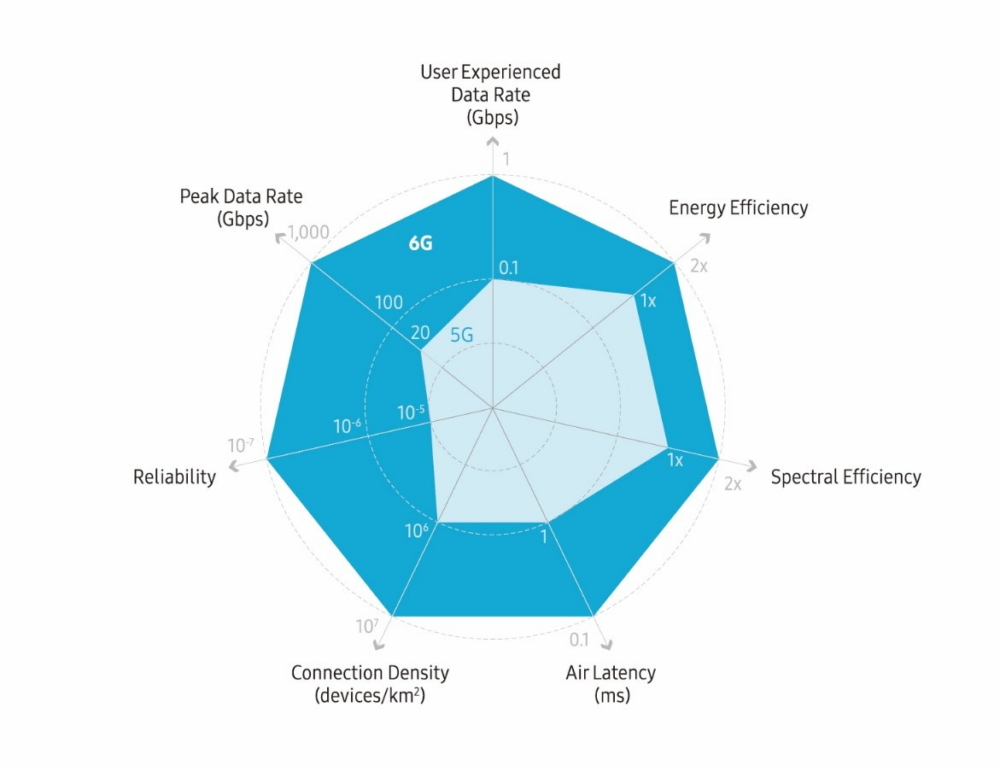
\includegraphics[width=0.71\textwidth]{samsung-6g.jpg}
  \vspace*{-0.5cm}
  \caption{Comparison of 5G and 6G performances. Source: Samsung Electronics\,\cite{samsungwhitepaper}}
  \label{fig:6g}
\end{figure}


\subsection{Security Technology}
%With the advent of innovative new ideas in 4IR, new security issues arise as well. We first need the 5G communication networks and IoT devices to be reliable\,\cite{presidential2019}. For example, in self driving, a temporary disconnect in communication may result in traffic interference, or even life-threatening accidents can occur due to hacking. We also need to prepare for new technologies that break existing security technologies. As the number of IoT devices increases, DDoS (Distributed Denial-of-Service attack) attacks using those devices become easier\,\cite{ddos2016}. In addition, we need to prepare for the vulnerability of asymmetric keys (RSA\,\cite{DBLP:journals/cacm/RivestSA83} and ECC\,\cite{Koblitz1987,DBLP:conf/crypto/Miller85}) against quantum computers\,\cite{presidential2019}. While cyber security is critical in 4IR\,\cite{10.5555/3312394}, we should also make sure it does not stall progress.

%The following quote can be found at the end of the recommendations made by the Korean Presidential Committee on 4IR on October 25th, 2019.
%``As Klaus Schwab revealed in his book ‘The Next’, if cyber security is not guaranteed, all attempts related to 4IR will be like a castle built on sand, which cannot last long. However, security should not become a regulation either. Only when we find a balance between the dilemmas will Korea have a credible status as a hyper-connected nation.’’ Source: Daily Secu (https://www.dailysecu.com) 

A core technology of 4IR, security technology is inextricably related to the other core technologies---big data, AI, and IoT. In this section, we discuss the security issues in each of these three. 

\subsubsection{Security in Big Data}

\begin{itemize}
  \item Data protection and privacy preserving: 
  % As mentioned before, data becomes extremely variable assets as the oil in 4IR era, therefore they are needed to be strictly protected. Privacy preserving also becomes crucial concerns for individuals and societies due to prevalent threat to personal information. 
  Big data poses new threats in data protection and privacy beyond what traditional cryptography and de-identification techniques could counter. For example,
  existing de-identification techniques including $k$-anonymity\,\cite{Sweeney2013} and $l$-diversity\,\cite{Machanavajjhala2006} may be vulnerable to re-identification attacks\,\cite{Henriksen-Bulmer2016}. Thus, differential privacy\,\cite{Cynthia2014} is being considered as an alternative to preserve privacy. \emph{Differential privacy} enables us to publicly share a dataset by conserving statistical properties of groups in the dataset while hiding exact information about individuals in it. Differential privacy has been widely used in collecting and analyzing big data, e.g., by U.S. Census Bureau for showing commuting patterns\,\cite{Ashwin2008}, Google for sharing historical traffic statistics\,\cite{Google2015}, Apple for improving the intelligent personal assistant technology of iOS 10\,\cite{Apple2016}, and Microsoft for implementing telemetry in Windows\,\cite{Bolin2017}. 
  Meanwhile, fast evolution of computing power mainly driven by quantum computing may invalidate existing cryptography systems whose safety is supposed to be guaranteed by extremely high computational complexity\,\cite{bernstein2009introduction}. \emph{Quantum cryptography}\,\cite{Nicolas2002}, in which copying and viewing encrypted message without notification is impossible, can be considered as a countermeasure.
%PPDB deals with obtaining true data mining results without disclosing the basic sensitive data values.

  \item Security in distributed and decentralized information technology\,(IT) infrastructure: In the 4IR era, IT environments become more distributed and decentralized as distributed information processing engines such as Hadoop and Spark are widely used to handle large-scale data, and the IT service platforms move to cloud environments. 
  %To protect such distributed software and hardware infrastructure, traditional countermeasures such as intrusion detection, network security, identity and access management\,(IAM), and distributed denial-of-service\,(DDos) protection have been redesigned. 
  To protect such distributed IT infrastructure, identity and access management\,(IAM), data loss prevention\,(DLP), security information and event management\,(SIEM), business continuity and disaster recovery\,(BCDR) are considered as common countermeasures\,\cite{cloudSecurity} along with traditional cybersecurity techniques such as intrusion detection, network security, and distributed denial-of-service\,(DDoS) protection.
  In addition, a virtualization technique, which securely separates multiple users on a single physical machine, plays a key role to ensure cybersecurity in distributed IT infrastructure, because it is common to share the same resource\,(e.g., machine) with multiple users\,\cite{Darshan2020}. 
%Virtual Machines(VMs) share the underlying hardware and rely on the software level isolation. Several security threats, risks, and vulnerabilities such as malicious VM images, sensitive data leakage, unsecured VM migrations in multi-cloud environments, and backdoor of host OS exist in present virtualization infrastructure that an adversary can utilize to infiltrate the security and privacy of the systems in cloud computing environments. 
Besides, a blockchain is expected to be an important technique to build a decentralized, trustworthy infrastructure even with presence of untrustworthy participants\,\cite{blockchain}. It is being widely used for cryptocurrency and smart contracts.

  \item Security in VR\,/\,AR: % VR/AR can cause serious security issues as it is applied to real life in near future\,\cite{SecurityARVR}. 
  VR\,/\,AR collects a much larger amount of private information about users and their behaviors compared to traditional input devices\,(e.g., keyboards and mouses) and social networking services\,(e.g., Facebook and Twitter)\,\cite{SecurityARVR}. Thus, with smartly forged content, VR\,/\,AR can be powerful means of spreading fake news and social prejudice. At the same time, the guarantee of its availability is crucial when it is utilized in mission-critical tasks such as life rescue, dron control, and production management. We also need to prepare for new security issues such as information sharing between VR\,/\,AR headsets and device protection with physiological or biometric information\,\cite{Guzman2019}.
  % interaction protection such as non-repudiation, authorization, authentication, identifiability, and policy/consent compliance
\end{itemize}


\subsubsection{Security in ML}

ML works with two valuable assets to be protected---data and models, where the former is the input of training and the latter the result. Attack on data is often referred to as \emph{data corruption} or \emph{data poisoning}\,\cite{AIMLThreat}. If the training data is unreliable or biased, ML generates models which may lead to false or unfair decisions. Data corruption or poisoning attacks intentionally manipulate the training data to deceive a model. In principle, such kind of attacks can be prevented with strict access control, confidential data storage, and cryptography. However, the nature of ML training data that a large volume comes from various sources makes this issue more complicated\,\cite{Sarker2020}. In addition, data extraction or exfiltration should be prevented because the training data can be used to infer the behavior of a trained model and can contain proprietary and private information\,\cite{Gary2019}. Attack on a model is often referred to as \emph{model manipulation} or \emph{backdooring} which publishes a model forged for potentially conducting malicious behaviors\,\cite{Gu2017}. The resulting service of such an inflicted model could be problematic. Like data extraction, a model can also be extracted to guess the prediction of the model or to find the hidden parameters influencing the prediction\,\cite{Gary2019}.

%Examples include theft of a proprietary model and enabling attacks on what was designed to be a model. 

\subsubsection{Security in Communications}


In the hyper-connected society realized by 4IR, the cyberattack surface is expanded to all the devices connected to the network---including computers, mobile devices, vehicles, wearable devices, appliances, sensors, and so on\,\cite{forbes2021}. Cyberattacks can target not only the communication between these devices but also the devices themselves. Regarding the IoT communication, lack of IoT security standards is regarded as one of the main obstacles\,\cite{Karie2021}. Because IoT communication is commonly applied to collect and transmit the information in many mission critical scenarios such as self driving, smart factories, and smart healthcare, even a short miscommunication or disconnection by an attack can cause significant damages\,\cite{Moore2020}. 
%For example, when a piece of forged information is delivered to self-driving cars, life-threatening accidents may happen. 
%Regarding the IoT devices, it is possible to trigger false instructions, steal the IoT devices, move the IoT devices to an unauthorized location, comprise the devices on the IoT terminal, and steal or tamper the information
% -->
Pervasive IoT devices also can be exposed to physical threats such as stealing,  unauthorized moving, compromising to steal information or inject forged data, and triggering false instructions that may cause malfunction\,\cite{Xiao2013}. 
%
In addition, traditional DDoS attacks become easier as the number of the devices that can be targeted increases on the IoT platform\,\cite{ddos2016}. 

\begin{comment}
4IR's hyper-connected society connects everything in real time with 5G wireless communication network. Connect everything nature of 5G network considerably expands the cyberattack surface which is all the network connected devices that can be exploited by attackers such as computers, mobile devices, vehicles, wearable devices, appliances, and sensors\,\cite{forbes2021}. Moreover, lack of IoT security standards in 5G network makes the security problems worse. Most of all, 5G networks should be reliable \,\cite{presidential2019}. For example, M2M with 5G network is applied to collect, transmit and manage the information especially in many mission critical scenarios such as Vehicle to Vehicle (V2V), smart grid, smart factory, and SCADA(Supervisory Control And Data Acquisition)\,\cite{Xiao2013}. In self driving with V2V, a temporary disconnect in communication among vehicles due to unreliable 5G network may result in traffic interference, or even life-threatening accidents. Aside from 5G networks, cyber security threats of IoT include false trigger instruction which will active a node incorrectly, stealing the IoT devices, moving the IoT devices to unauthorized location, node compromising attack in the IoT terminal layer, and stealing or tampering the information. We also need to concern the traditional DDoS (Distributed Denial-of-Service attack) attacks become easier as the number of IoT devices that can be participated for the attack increases\,\cite{ddos2016}.
\end{comment}

%5G network is dynamic software-based system which has far more traffic routing points than the current hardware-based, centralized hub-and-spoke designs that 4G has. 
%Many IoT devices are being manufactured with minimal or non-existent cybersecurity measures. These devices are already being used by hackers as entry points to enterprise networks.


\section{Example Application Technology: Molecular Biology}

AI has been actively used in molecular biology, especially for predicting protein structures. Google's DeepMind, well known as the inventor of AlphaGo, created AlphaFold\,\cite{AlphaFold}, the cutting edge AI network for predicting protein structures. Knowing how proteins fold is very useful for scientists to understand the biological processes of every creature. This direction of research can greatly impact on every field of molecular biology, from helping overcome disease and quickly discovering new medicines to revealing the mysteries of life.

% subset of machine learning in which multilayered neural networks learn from vast amounts of data.

Consistent with the trend of 4IR, \emph{deep learning}, a subset of ML in which deep\,(i.e., multilayered) neural networks learn from vast amounts of data, is attracting more and more attention in molecular biology as well. Notably, deep learning relieves the need for rigorous feature engineering done by domain experts, because a deep neural network itself can accept high-dimensional input as well as decide the importance of each feature and derive latent features\,\cite{Jisna2021}. Directly using raw input data without help from domain experts not only automates and speeds up the entire process but also increases the scalability of the input data. This benefit stands out especially in the 4IR era, because deep learning can digest unprecedented amounts of big data generated by DNA sequencing. 
For example, DeepTFactor\,\cite{DeepTFactor} is designed to predict a \emph{transcription factor\,(TF)}, which is a protein that specifically binds to DNA and regulates gene transcription. Identifying TFs is regarded as the starting point of the inspection of transcriptional regulatory systems\,\cite{DeepTFactor}. As shown in Figure \ref{fig:DeepTFactor}, DeepTFactor, which consists of convolutional neural networks (CNNs),  receives a protein sequence and predicts whether the given protein sequence is a TF. Three CNNs with different filter sizes can learn diverse latent features, and their outputs are concatenated to exploit all of these latent features; then, another CNN learns the mapping between the latent features and the class label\,(i.e., TF or non-TF). As a result, DeepTFactor achieves higher accuracy than previous TF classification tools\,\cite{DeepTFactor}. Overall, deep learning has become a powerful tool for various studies in molecular biology\,\cite{Webb2018}.

\begin{figure}[h]
  \centering
  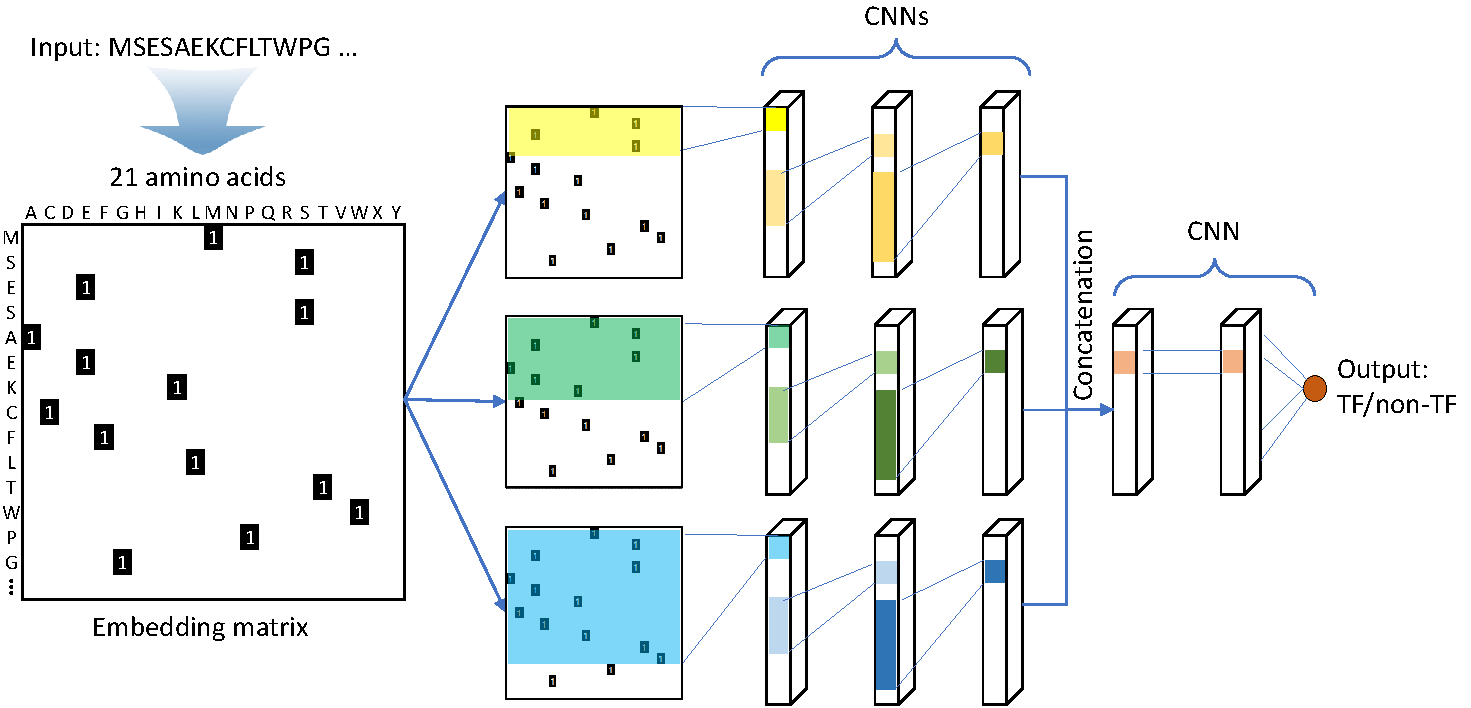
\includegraphics[width=0.9\textwidth]{DeepTFactor.pdf}
  \caption{Deep neural network architecture of DeepTFactor. A shade color indicates the connection between the input and output of a convolution operation. Source: Kim et al.\,\cite{DeepTFactor}}
  \label{fig:DeepTFactor}
\end{figure}


\section{Conclusion}
In summary, we categorized the various technologies in 4IR and covered important core technologies---big data, AI, IoT, and security. In addition, we presented an application of AI in molecular biology. We hope this article will serve as a useful stepping stone for a comprehensive understanding of the technologies related to 4IR.

\section*{Acknowledgment}
The authors deeply appreciate the invaluable help from Steven E. Whang in completing Section 4.1.

\bibliographystyle{plain}
\small
\itemsep=1pt
%\bibliography{references}

\begin{thebibliography}{10}

\bibitem{6g}
6{G} (network).
\newblock \url{https://en.wikipedia.org/wiki/6G_(network)}.
\newblock Accessed June 12th, 2022.

\bibitem{Apple2016}
Apple previews {iOS} 10, the biggest {iOS} release ever.
\newblock
  \url{https://www.apple.com/newsroom/2016/06/apple-previews-ios-10-biggest-ios-release-ever/}.
\newblock Accessed June 15th, 2022.

\bibitem{blockchain}
Blockchain in {W}ikipedia.
\newblock \url{https://en.wikipedia.org/wiki/Blockchain}.
\newblock Accessed June 15th, 2022.

\bibitem{iste2016}
Computational thinking.
\newblock \url{http://www.iste.org/standards/standards/for-students-2016}.
\newblock Accessed June 10th, 2022.

\bibitem{wiki-computational-thinking}
Computational thinking.
\newblock \url{https://en.wikipedia.org/wiki/Computational_thinking}.
\newblock Accessed June 10th, 2022.

\bibitem{data-centric-ai}
Data-centric {AI}.
\newblock \url{https://datacentricai.org/}.
\newblock Accessed June 5th, 2022.

\bibitem{ddos2016}
Ddos attack that disrupted internet was largest of its kind in history, experts
  say.
\newblock
  \url{https://www.theguardian.com/technology/2016/oct/26/ddos-attack-dyn-mirai-botnet}.
\newblock Accessed June 10th, 2022.

\bibitem{compas}
How we analyzed the compas recidivism algorithm.
\newblock
  \url{https://www.propublica.org/article/how-we-analyzed-the-compas-recidivism-algorithm}.
\newblock Accessed June 5th, 2022.

\bibitem{Hyundai2022}
Hyundai motor company's mid-to-long term electrification strategy disclosed (in
  {K}orean).
\newblock \url{https://www.hyundai.co.kr/news/CONT0000000000012239}.
\newblock Accessed August 1st, 2022.

\bibitem{ioe}
Internet of everything.
\newblock
  \url{https://www.techtarget.com/iotagenda/definition/Internet-of-Everything-IoE}.
\newblock Accessed June 10th, 2022.

\bibitem{iot}
Internet of things.
\newblock \url{https://www.oracle.com/internet-of-things/what-is-iot/}.
\newblock Accessed June 10th, 2022.

\bibitem{BBC2022}
Introduction to computational thinking.
\newblock \url{https://www.bbc.co.uk/bitesize/guides/zp92mp3/revision/1}.
\newblock Accessed June 5th, 2022.

\bibitem{Reuters2022}
The long road to electric cars.
\newblock \url{https://graphics.reuters.com/AUTOS-ELECTRIC/USA/mopanyqxwva/}.
\newblock Accessed August 1st, 2022.

\bibitem{Schwab2016b}
Schwab {K}laus. {T}he fourth industrial revolution: what it means, how to
  respond.
\newblock
  \url{https://www.weforum.org/agenda/2016/01/the-fourth-industrial-revolution-what-it-means-and-how-to-respond/}.
\newblock World Economic Forum, June 2016.

\bibitem{SecurityARVR}
The security risks of {AR} and {VR}.
\newblock \url{ https://defpr.com/the-security-risks-of-ar-and-vr/}.
\newblock Accessed June 15th, 2022.

\bibitem{leeluda}
A {S}outh {K}orean chatbot shows just how sloppy tech companies can be with
  user data.
\newblock
  \url{https://slate.com/technology/2021/04/scatterlab-lee-luda-chatbot-kakaotalk-ai-privacy.html}.
\newblock Accessed June 5th, 2022.

\bibitem{Google2015}
Tackling urban mobility with technology.
\newblock
  \url{https://europe.googleblog.com/2015/11/tackling-urban-mobility-with-technology.html}.
\newblock Accessed June 15th, 2022.

\bibitem{AIMLThreat}
Top 5 security threats facing artificial intelligence and machine learning.
\newblock
  \url{https://hubsecurity.com/blog/cyber-security/security-threats-for-ai-and-machine-learning/}.
\newblock Accessed June 15th, 2022.

\bibitem{trustworthy-ai}
Trustworthy {AI}.
\newblock \url{https://www.ibm.com/watson/trustworthy-ai}.
\newblock Accessed June 5th, 2022.

\bibitem{cloudSecurity}
What is cloud security?
\newblock \url{https://www.ibm.com/topics/cloud-security}.
\newblock Accessed July 25th, 2022.

\bibitem{forbes2021}
Why {5G} networks are disrupting the cybersecurity industry.
\newblock
  \url{https://www.forbes.com/sites/forbestechcouncil/2021/10/29/why-5g-networks-are-disrupting-the-cybersecurity-industry/?sh=4b997d5a1fe9}.
\newblock Accessed June 15th, 2022.

\bibitem{10.1145/1929887.1929905}
Valerie Barr and Chris Stephenson.
\newblock Bringing computational thinking to {K}-12: What is involved and what
  is the role of the computer science education community?
\newblock {\em ACM Inroads}, 2(1):48--54, February 2011.

\bibitem{DBLP:conf/kdd/BaylorBCFFHHIJK17}
Denis Baylor, Eric Breck, Heng{-}Tze Cheng, Noah Fiedel, Chuan~Yu Foo, Zakaria
  Haque, Salem Haykal, Mustafa Ispir, Vihan Jain, Levent Koc, Chiu~Yuen Koo,
  Lukasz Lew, Clemens Mewald, Akshay~Naresh Modi, Neoklis Polyzotis, Sukriti
  Ramesh, Sudip Roy, Steven~Euijong Whang, Martin Wicke, Jarek Wilkiewicz, Xin
  Zhang, and Martin Zinkevich.
\newblock {TFX:} {A} tensorflow-based production-scale machine learning
  platform.
\newblock In {\em KDD}, pages 1387--1395. {ACM}, 2017.

\bibitem{bernstein2009introduction}
Daniel~J Bernstein.
\newblock Introduction to post-quantum cryptography.
\newblock In {\em Post-quantum cryptography}, pages 1--14. Springer, 2009.

\bibitem{Berry14}
Miles Berry.
\newblock This is for everyone {K}12 computer science in {E}ngland.
\newblock In {\em The 21st KAST International Symposium (KAST 20th Anniversary
  International Symposium), Plaza Hotel, Seoul}, 2014.

\bibitem{DBLP:conf/cidr/BoehmADGIKLPR20}
Matthias Boehm, Iulian Antonov, Sebastian Baunsgaard, Mark Dokter, Robert
  Ginth{\"{o}}r, Kevin Innerebner, Florijan Klezin, Stefanie~N. Lindstaedt,
  Arnab Phani, Benjamin Rath, Berthold Reinwald, Shafaq Siddiqui, and
  Sebastian~Benjamin Wrede.
\newblock Systemds: {A} declarative machine learning system for the end-to-end
  data science lifecycle.
\newblock In {\em CIDR}, 2020.

\bibitem{DBLP:conf/icde/ChaudhuriFB99}
Surajit Chaudhuri, Usama~M. Fayyad, and Jeff Bernhardt.
\newblock Scalable classification over {SQL} databases.
\newblock In {\em ICDE}, pages 470--479. {IEEE}, 1999.

\bibitem{DBLP:journals/pvldb/ChenKNP17}
Lingjiao Chen, Arun Kumar, Jeffrey~F. Naughton, and Jignesh~M. Patel.
\newblock Towards linear algebra over normalized data.
\newblock {\em Proc. {VLDB} Endow.}, 10(11):1214--1225, 2017.

\bibitem{Guzman2019}
Jaybie~A. de~Guzman, Kanchana Thilakarathna, and Aruna Seneviratne.
\newblock Security and privacy approaches in mixed reality: {A} literature
  survey.
\newblock {\em {ACM} Comput. Surv.}, 52(6):110:1--110:37, 2020.

\bibitem{DBLP:books/sp/17/DelckerI17}
Jan Delcker and Dirk Ifenthaler.
\newblock Computational thinking as an interdisciplinary approach to computer
  science school curricula: {A} {G}erman perspective.
\newblock In Peter~J. Rich and Charles~B. Hodges, editors, {\em Emerging
  Research, Practice, and Policy on Computational Thinking}, pages 49--62.
  Springer, 2017.

\bibitem{DBLP:journals/cacm/DenningTY17}
Peter~J. Denning, Matti Tedre, and Pat Yongpradit.
\newblock Misconceptions about computer science.
\newblock {\em Commun. {ACM}}, 60(3):31--33, 2017.

\bibitem{Bolin2017}
Bolin Ding, Janardhan Kulkarni, and Sergey Yekhanin.
\newblock Collecting telemetry data privately.
\newblock In {\em NeurIPS}, pages 3571--3580, 2017.

\bibitem{DBLP:conf/sigmod/DingMYWDLZCGKLK20}
Jialin Ding, Umar~Farooq Minhas, Jia Yu, Chi Wang, Jaeyoung Do, Yinan Li,
  Hantian Zhang, Badrish Chandramouli, Johannes Gehrke, Donald Kossmann,
  David~B. Lomet, and Tim Kraska.
\newblock {ALEX:} an updatable adaptive learned index.
\newblock In {\em SIGMOD}, pages 969--984. {ACM}, 2020.

\bibitem{Cynthia2014}
Cynthia Dwork and Aaron Roth.
\newblock The algorithmic foundations of differential privacy.
\newblock {\em Found. Trends Theor. Comput. Sci.}, 9(3-4):211--407, 2014.

\bibitem{Nicolas2002}
Nicolas Gisin, Gr\'egoire Ribordy, Wolfgang Tittel, and Hugo Zbinden.
\newblock Quantum cryptography.
\newblock {\em Rev. Mod. Phys.}, 74:145--195, March 2002.

\bibitem{Gu2017}
Tianyu Gu, Brendan Dolan{-}Gavitt, and Siddharth Garg.
\newblock Badnets: Identifying vulnerabilities in the machine learning model
  supply chain.
\newblock {\em CoRR}, abs/1708.06733, 2017.

\bibitem{Henriksen-Bulmer2016}
Jane Henriksen{-}Bulmer and Sheridan Jeary.
\newblock Re-identification attacks--{A} systematic literature review.
\newblock {\em Int. J. Inf. Manag.}, 36(6):1184--1192, 2016.

\bibitem{Jisna2021}
V.A. Jisna and P.B. Jayaraj.
\newblock Protein structure prediction: Conventional and deep learning
  perspectives.
\newblock {\em Protein Journal}, 40:522--544, 2021.

\bibitem{AlphaFold}
John Jumper et~al.
\newblock Highly accurate protein structure prediction with {AlphaFold}.
\newblock {\em Nature}, 596:583--589, 2021.

\bibitem{Karie2021}
Nickson~M. Karie, Nor~Masri Sahri, Wencheng Yang, Craig Valli, and Victor~R.
  Kebande.
\newblock A review of security standards and frameworks for {I}o{T}-based smart
  environments.
\newblock {\em {IEEE} Access}, 9:121975--121995, 2021.

\bibitem{DeepTFactor}
Gi~Bae Kim, Ye~Gao, Bernhard~O. Palsson, and Sang~Yup Lee.
\newblock {DeepTFactor}: A deep learning-based tool for the prediction of
  transcription factors.
\newblock {\em Proceedings of the National Academy of Sciences of the United
  States of America (PNAS)}, 118(2):e2021171118, 2021.

\bibitem{DBLP:journals/debu/KraskaM0PPRS21}
Tim Kraska, Umar~Farooq Minhas, Thomas Neumann, Olga Papaemmanouil, Jignesh~M.
  Patel, Christopher R{\'{e}}, and Michael Stonebraker.
\newblock {ML}-in-databases: Assessment and prognosis.
\newblock {\em {IEEE} Data Eng. Bull.}, 44(1):3--10, 2021.

\bibitem{lasi2014industry}
Heiner Lasi, Peter Fettke, Hans-Georg Kemper, Thomas Feld, and Michael
  Hoffmann.
\newblock Industry 4.0.
\newblock {\em Business \& information systems engineering}, 6(4):239--242,
  2014.

\bibitem{DBLP:journals/pvldb/LiZLG19}
Guoliang Li, Xuanhe Zhou, Shifu Li, and Bo~Gao.
\newblock Qtune: {A} query-aware database tuning system with deep reinforcement
  learning.
\newblock {\em Proc. {VLDB} Endow.}, 12(12):2118--2130, 2019.

\bibitem{DBLP:conf/icde/LiRBZCZ21}
Peng Li, Xi~Rao, Jennifer Blase, Yue Zhang, Xu~Chu, and Ce~Zhang.
\newblock Clean{ML}: {A} study for evaluating the impact of data cleaning on
  {ML} classification tasks.
\newblock In {\em ICDE}, pages 13--24. {IEEE}, 2021.

\bibitem{Machanavajjhala2006}
Ashwin Machanavajjhala, Johannes Gehrke, Daniel Kifer, and Muthuramakrishnan
  Venkitasubramaniam.
\newblock l-diversity: privacy beyond k-anonymity.
\newblock In {\em ICDE}, pages 24--35. IEEE, 2006.

\bibitem{Ashwin2008}
Ashwin Machanavajjhala, Daniel Kifer, John~M. Abowd, Johannes Gehrke, and Lars
  Vilhuber.
\newblock Privacy: Theory meets practice on the map.
\newblock In {\em ICDE}, pages 277--286. IEEE, 2008.

\bibitem{DBLP:journals/pvldb/MarcusNMZAKPT19}
Ryan~C. Marcus, Parimarjan Negi, Hongzi Mao, Chi Zhang, Mohammad Alizadeh, Tim
  Kraska, Olga Papaemmanouil, and Nesime Tatbul.
\newblock Neo: {A} learned query optimizer.
\newblock {\em Proc. {VLDB} Endow.}, 12(11):1705--1718, 2019.

\bibitem{Gary2019}
Gary McGraw, Richie Bonett, Harold Figueroa, and Victor Shepardson.
\newblock Security engineering for machine learning.
\newblock {\em Computer}, 52(8):54--57, 2019.

\bibitem{DBLP:journals/cacm/MolinoR22}
Piero Molino and Christopher R{\'{e}}.
\newblock Declarative machine learning systems.
\newblock {\em Commun. {ACM}}, 65(1):42--49, 2022.

\bibitem{Moore2020}
Samuel~J. Moore, Chris~D. Nugent, Shuai Zhang, and Ian Cleland.
\newblock Io{T} reliability: a review leading to 5 key research directions.
\newblock {\em {CCF} Trans. Pervasive Comput. Interact.}, 2(3):147--163, 2020.

\bibitem{Xiao2013}
Xiao Nie and Xiaobing Zhai.
\newblock {M2M} security threat and security mechanism research.
\newblock In {\em ICCSNT}, pages 906--909, 2013.

\bibitem{DBLP:journals/sigmod/PolyzotisRWZ18}
Neoklis Polyzotis, Sudip Roy, Steven~Euijong Whang, and Martin Zinkevich.
\newblock Data lifecycle challenges in production machine learning: {A} survey.
\newblock {\em {SIGMOD} Rec.}, 47(2):17--28, 2018.

\bibitem{DBLP:journals/vldb/RatnerBEFWR20}
Alexander Ratner, Stephen~H. Bach, Henry~R. Ehrenberg, Jason~A. Fries, Sen Wu,
  and Christopher R{\'{e}}.
\newblock Snorkel: rapid training data creation with weak supervision.
\newblock {\em {VLDB} J.}, 29(2-3):709--730, 2020.

\bibitem{DBLP:books/sp/RH2017}
Peter~J. Rich and Charles~B. Hodges, editors.
\newblock {\em Emerging Research, Practice, and Policy on Computational
  Thinking}.
\newblock Springer, 2017.

\bibitem{Rifkin2011}
Jeremy Rifkin.
\newblock {\em The Third Industrial Revolution}.
\newblock Palgrave MacMillan, 2011.

\bibitem{DBLP:journals/tkde/RohHW21}
Yuji Roh, Geon Heo, and Steven~Euijong Whang.
\newblock A survey on data collection for machine learning: {A} {B}ig data -
  {AI} integration perspective.
\newblock {\em {IEEE} Trans. Knowl. Data Eng.}, 33(4):1328--1347, 2021.

\bibitem{samsung2019}
Samsung.
\newblock {5G} launches in {K}orea.
\newblock
  \url{https://images.samsung.com/is/content/samsung/p5/global/business/networks/insights/white-paper/5g-launches-in-korea-get-a-taste-of-the-future/5G-Launches-in-Korea-Get-a-taste-of-the-future.pdf}.
\newblock 2019.

\bibitem{samsung2018}
Samsung.
\newblock Who \& {H}ow: making {5G} {NR} standards.
\newblock
  \url{https://images.samsung.com/is/content/samsung/p5/global/business/networks/insights/white-paper/who-and-how_making-5g-nr-standards/who-and-how_making-5g-nr-standards.pdf}.
\newblock 2018.

\bibitem{samsungwhitepaper}
Samsung.
\newblock 6{G} the next hyper-connected experience for all.
\newblock White paper, Samsung Research, 2020.

\bibitem{Sarker2020}
Iqbal~H. Sarker, A.~S.~M. Kayes, Shahriar Badsha, Hamed AlQahtani, Paul~A.
  Watters, and Alex Ng.
\newblock Cybersecurity data science: an overview from machine learning
  perspective.
\newblock {\em J. Big Data}, 7(1):1--29, 2020.

\bibitem{Schwab2016}
Klaus Schwab.
\newblock {\em The Fourth Industrial Revolution}.
\newblock Portfolio Penguin, 2016.

\bibitem{DBLP:conf/nips/SculleyHGDPECYC15}
D.~Sculley, Gary Holt, Daniel Golovin, Eugene Davydov, Todd Phillips, Dietmar
  Ebner, Vinay Chaudhary, Michael Young, Jean{-}Fran{\c{c}}ois Crespo, and Dan
  Dennison.
\newblock Hidden technical debt in machine learning systems.
\newblock In {\em NeurIPS}, pages 2503--2511, 2015.

\bibitem{DBLP:conf/icml/SongK019}
Hwanjun Song, Minseok Kim, and Jae{-}Gil Lee.
\newblock {SELFIE:} refurbishing unclean samples for robust deep learning.
\newblock In {\em ICML}, pages 5907--5915. {PMLR}, 2019.

\bibitem{DBLP:journals/debu/StonebrakerR19}
Michael Stonebraker and El~Kindi Rezig.
\newblock Machine learning and {B}ig data: What is important?
\newblock {\em {IEEE} Data Eng. Bull.}, 42(4):3--7, 2019.

\bibitem{Sweeney2013}
Latanya Sweeney.
\newblock k-anonymity: A model for protecting privacy.
\newblock {\em Int. J. Uncertain. Fuzziness Knowl. Based Syst.},
  10(5):557--570, 2002.

\bibitem{Darshan2020}
Darshan Tank, Akshai Aggarwal, and Nirbhay Chaubey.
\newblock {\em Cyber Security Aspects of Virtualization in Cloud Computing
  Environments: Analyzing Virtualization-Specific Cyber Security Risks}, pages
  283--299.
\newblock January 2020.

\bibitem{rcrwireless}
Juan~Pedro Tomas.
\newblock South korea ends {F}ebruary with almost 203,000 5g base stations:
  Report.
\newblock
  \url{https://rcrwireless.com/20220331/5g/south-korea-ends-february-almost-203000-5g-base-stations-report},
  March 2022.

\bibitem{DBLP:journals/debu/Ullman20}
Jeffrey~D. Ullman.
\newblock The battle for data science.
\newblock {\em {IEEE} Data Eng. Bull.}, 43(2):8--14, 2020.

\bibitem{Webb2018}
Sarah Webb.
\newblock Deep learning for biology.
\newblock {\em Nature}, 554:555--557, 2018.

\bibitem{DBLP:journals/cacm/Wing06}
Jeannette~M. Wing.
\newblock Computational thinking.
\newblock {\em Commun. {ACM}}, 49(3):33--35, 2006.

\bibitem{Wirth1976}
Niklaus Wirth.
\newblock {\em Algorithms + Data Structures = Programs}.
\newblock Prentice-Hall, 1976.

\end{thebibliography}


\end{document}
